\documentclass{standalone}
\usepackage{tikz,pgfplots}
\pgfplotsset{compat = 1.18}

\begin{document}
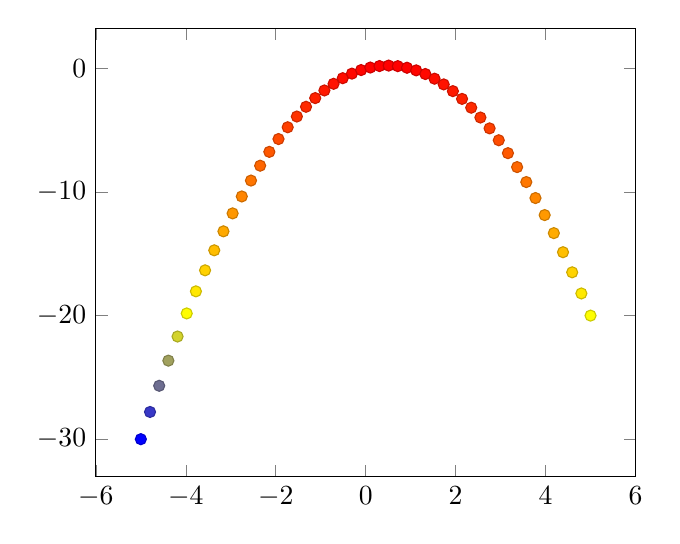
\begin{tikzpicture}
\begin{axis}
% scatter src=none|<expression>|x|y|z|f(x)|explicit|explicit symbolic
\addplot+ [
    scatter,
    only marks,
    samples=50,
    scatter src=y,
] {x - x^2};
\end{axis}
\end{tikzpicture}


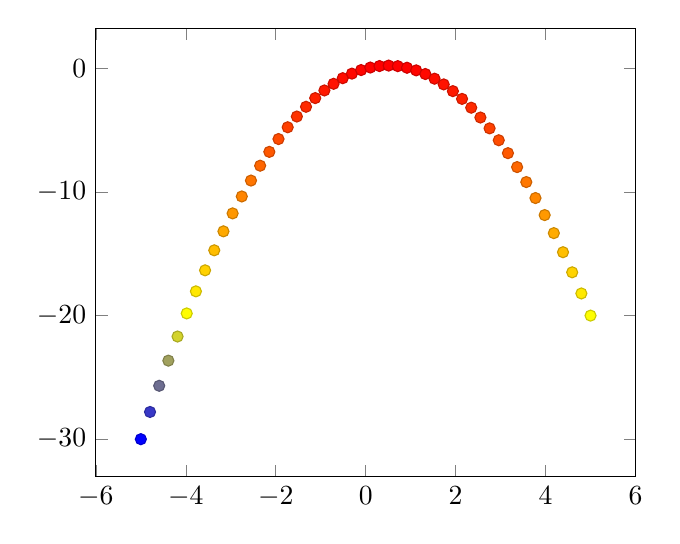
\begin{tikzpicture}
\begin{axis}
% scatter src=none|<expression>|x|y|z|f(x)|explicit|explicit symbolic
\addplot+ [
    scatter,
    only marks,
    samples=50,
    scatter src=f(x),
] {x - x^2};
\end{axis}
\end{tikzpicture}


\begin{tikzpicture}
\begin{axis}
% scatter src=none|<expression>|x|y|z|f(x)|explicit|explicit symbolic
\addplot+ [
    scatter,
    only marks,
    scatter src=explicit]
coordinates {
    (0,0) [1.0e10]
    (1,2) [1.1e10]
    (2,3) [1.2e10]
    (3,4) [1.3e10]
    };
\end{axis}
\end{tikzpicture}


\end{document}